\documentclass[12pt, titlepage]{article}

\usepackage{booktabs}
\usepackage{tabularx}
\usepackage{hyperref}
\hypersetup{
    colorlinks,
    citecolor=black,
    filecolor=black,
    linkcolor=red,
    urlcolor=blue
}
\usepackage[round]{natbib}
\usepackage{graphicx}


%% Comments

\usepackage{color}

%\newif\ifcomments\commentstrue %displays comments
\newif\ifcomments\commentsfalse %so that comments do not display

\ifcomments
\newcommand{\authornote}[3]{\textcolor{#1}{[#3 ---#2]}}
\newcommand{\todo}[1]{\textcolor{red}{[TODO: #1]}}
\else
\newcommand{\authornote}[3]{}
\newcommand{\todo}[1]{}
\fi

\newcommand{\wss}[1]{\authornote{blue}{SS}{#1}} 
\newcommand{\plt}[1]{\authornote{magenta}{TPLT}{#1}} %For explanation of the template
\newcommand{\an}[1]{\authornote{cyan}{Author}{#1}}

%% Common Parts

\newcommand{\progname}{Inverted Pendulum Control Systems} % PUT YOUR PROGRAM NAME HERE
\newcommand{\authname}{Morteza Mirzaei} % AUTHOR NAMES                  

\usepackage{hyperref}
    \hypersetup{colorlinks=true, linkcolor=blue, citecolor=blue, filecolor=blue,
                urlcolor=blue, unicode=false}
    \urlstyle{same}
                                


\begin{document}

\title{Verification and Validation Report:\\ \progname \\ (IPCS)} 
\author{\authname}
\date{\today}
	
\maketitle

\pagenumbering{roman}

\section{Revision History}

\begin{tabularx}{\textwidth}{p{3cm}p{2cm}X}
\toprule {\bf Date} & {\bf Version} & {\bf Notes}\\
\midrule
Date 1 & 1.0 & Notes\\
Date 2 & 1.1 & Notes\\
\bottomrule
\end{tabularx}

~\newpage

\section{Symbols, Abbreviations and Acronyms}

\renewcommand{\arraystretch}{1.2}
\begin{tabular}{l l} 
  \toprule		
  \textbf{symbol} & \textbf{description} \\
  \midrule 
  T               & Test                 \\
  UT              & Unit Test            \\
  \bottomrule
\end{tabular}\\

\wss{symbols, abbreviations or acronyms -- you can reference the SRS tables if needed}

\newpage

\tableofcontents

\listoftables %if appropriate

\listoffigures %if appropriate

\newpage

\pagenumbering{arabic}

This document reports the results of executing the
\href{https://github.com/mirzaim/ipcs/blob/main/docs/VnVPlan/VnVPlan.pdf}{VnV Plan}.

\section{Functional Requirements Evaluation}
This section covers the evaluation of the functional requirements.

\subsection{test-input-1}
This test checks if the software returns proper exceptions for invalid inputs 
and works properly for valid inputs. This test is implemented in 
the file \url{https://github.com/mirzaim/ipcs/blob/main/test/test_integration.py}, 
and the function name is \texttt{test\_input\_1}. The test passed successfully.

\begin{small}
  \begin{verbatim}
test_integration.py::test_input_1[0.0-0.0--90.0-16.0-80.0-1.0-False]  PASSED
test_integration.py::test_input_1[abc-0.0--90.0-16.0-80.0-1.0-True]   PASSED 
test_integration.py::test_input_1[0.0-abc--90.0-16.0-80.0-1.0-True]   PASSED 
test_integration.py::test_input_1[0.0-0.0-abc-16.0-80.0-1.0-True]     PASSED   
test_integration.py::test_input_1[0.0-0.0--90.0-abc-80.0-1.0-True]    PASSED  
test_integration.py::test_input_1[0.0-0.0--90.0-16.0-abc-1.0-True]    PASSED  
test_integration.py::test_input_1[0.0-0.0--90.0-16.0-80.0-abc-True]   PASSED 
test_integration.py::test_input_1[0.0-0.0--90.0--16.0-80.0-1.0-True]  PASSED
test_integration.py::test_input_1[0.0-0.0--90.0-16.0--80.0-1.0-True]  PASSED
test_integration.py::test_input_1[0.0-0.0--90.0-16.0-80.0--1.0-True]  PASSED
test_integration.py::test_input_1[0.0-0.0--90.0-100.0-80.0-1.0-True]  PASSED
test_integration.py::test_input_1[0.0-0.0--90.0-16.0-100.0-1.0-True]  PASSED
test_integration.py::test_input_1[0.0-0.0--90.0-16.0-80.0-50.0-True]  PASSED
test_integration.py::test_input_1[0.0-0.0--90.0-5.0-80.0-1.0-True]    PASSED  
test_integration.py::test_input_1[0.0-0.0--90.0-90.0-80.0-1.0-True]   PASSED 
test_integration.py::test_input_1[0.0--20.0--90.0-16.0-80.0-1.0-True] PASSED
test_integration.py::test_input_1[0.0-20.0--90.0-16.0-80.0-1.0-True]  PASSED
  \end{verbatim}
\end{small}

\subsection{test-sim-1}
This section focuses on testing the world simulator responsible for 
executing the inverted pendulum physics. 
The testing procedure involves verifying that given the initial 
position of the pendulum the location of the pendulum is accurately 
determined after a specified duration of time.
This test is implemented in 
the file \url{https://github.com/mirzaim/ipcs/blob/main/test/test_integration.py}, 
and the function name is \texttt{test\_sim\_1}. If the relative error
between the expected and actual values is less than $5\%$, the test is considered
successful. All the test passed successfully.

\begin{small}
  \begin{verbatim}
test_integration.py::test_sim_1[0.0-0.0--90.0-16.0-80.0-1.0-5.0-0.25]   PASSED 
test_integration.py::test_sim_1[0.0--5.0--90.0-16.0-80.0-1.0-5.0--4.75] PASSED
test_integration.py::test_sim_1[0.0-5.0--90.0-16.0-80.0-1.0-5.0-5.25]   PASSED 
test_integration.py::test_sim_1[0.0-0.0-0.0-16.0-80.0-1.0-6.0-0.08]     PASSED   
test_integration.py::test_sim_1[0.0-0.0--45.0-16.0-80.0-1.0-2.5--0.3]   PASSED 
test_integration.py::test_sim_1[0.0-0.0--90.0-30.0-80.0-1.0-1.5-0.8]    PASSED  
test_integration.py::test_sim_1[0.0-0.0--90.0-16.0-50.0-1.0-1.45-1.3]   PASSED 
test_integration.py::test_sim_1[0.0-0.0--90.0-16.0-80.0-20.0-5.0-0.25]  PASSED
test_integration.py::test_sim_1[5.0-0.0--90.0-16.0-80.0-1.0-2.7-0.65]   PASSED 
test_integration.py::test_sim_1[-5.0-0.0--90.0-16.0-80.0-1.0-5.5-0.0]   PASSED
  \end{verbatim}
\end{small}

\subsection{test-control-1}
The testing procedure involves verifying that given the initial
position of the pendulum the control system can keeping the pendulum
upright for 10 seconds after 30 seconds.
The test is implemented in the file 
\url{https://github.com/mirzaim/ipcs/blob/main/test/test_integration.py}
and the function name is \texttt{test\_control\_1}.
All the test passed successfully.

\begin{small}
  \begin{verbatim}
test_integration.py::test_control_1[0.0-0.0--90.0-16.0-80.0-1.0]  PASSED 
test_integration.py::test_control_1[0.0--5.0--90.0-16.0-80.0-1.0] PASSED
test_integration.py::test_control_1[0.0-5.0--90.0-16.0-80.0-1.0]  PASSED 
test_integration.py::test_control_1[0.0-0.0-0.0-16.0-80.0-1.0]    PASSED   
test_integration.py::test_control_1[0.0-0.0--45.0-16.0-80.0-1.0]  PASSED 
test_integration.py::test_control_1[0.0-0.0--90.0-30.0-80.0-1.0]  PASSED 
test_integration.py::test_control_1[0.0-0.0--90.0-16.0-50.0-1.0]  PASSED 
test_integration.py::test_control_1[0.0-0.0--90.0-16.0-80.0-20.0] PASSED
test_integration.py::test_control_1[5.0-0.0--90.0-16.0-80.0-1.0]  PASSED 
test_integration.py::test_control_1[-5.0-0.0--90.0-16.0-80.0-1.0] PASSED
  \end{verbatim}
\end{small}

\subsection{test-vis-1}
This test checks the correctness of the visualization. We took 4 screenshots
(\autoref{fig:test_vis_1_1}, \autoref{fig:test_vis_1_2}, \autoref{fig:test_vis_1_3}, 
and \autoref{fig:test_vis_1_4}) of the visualization with different inputs.
The correctness of the visualization is evaluated and all the test passed successfully.

\begin{figure}[h!]
  \begin{center}
    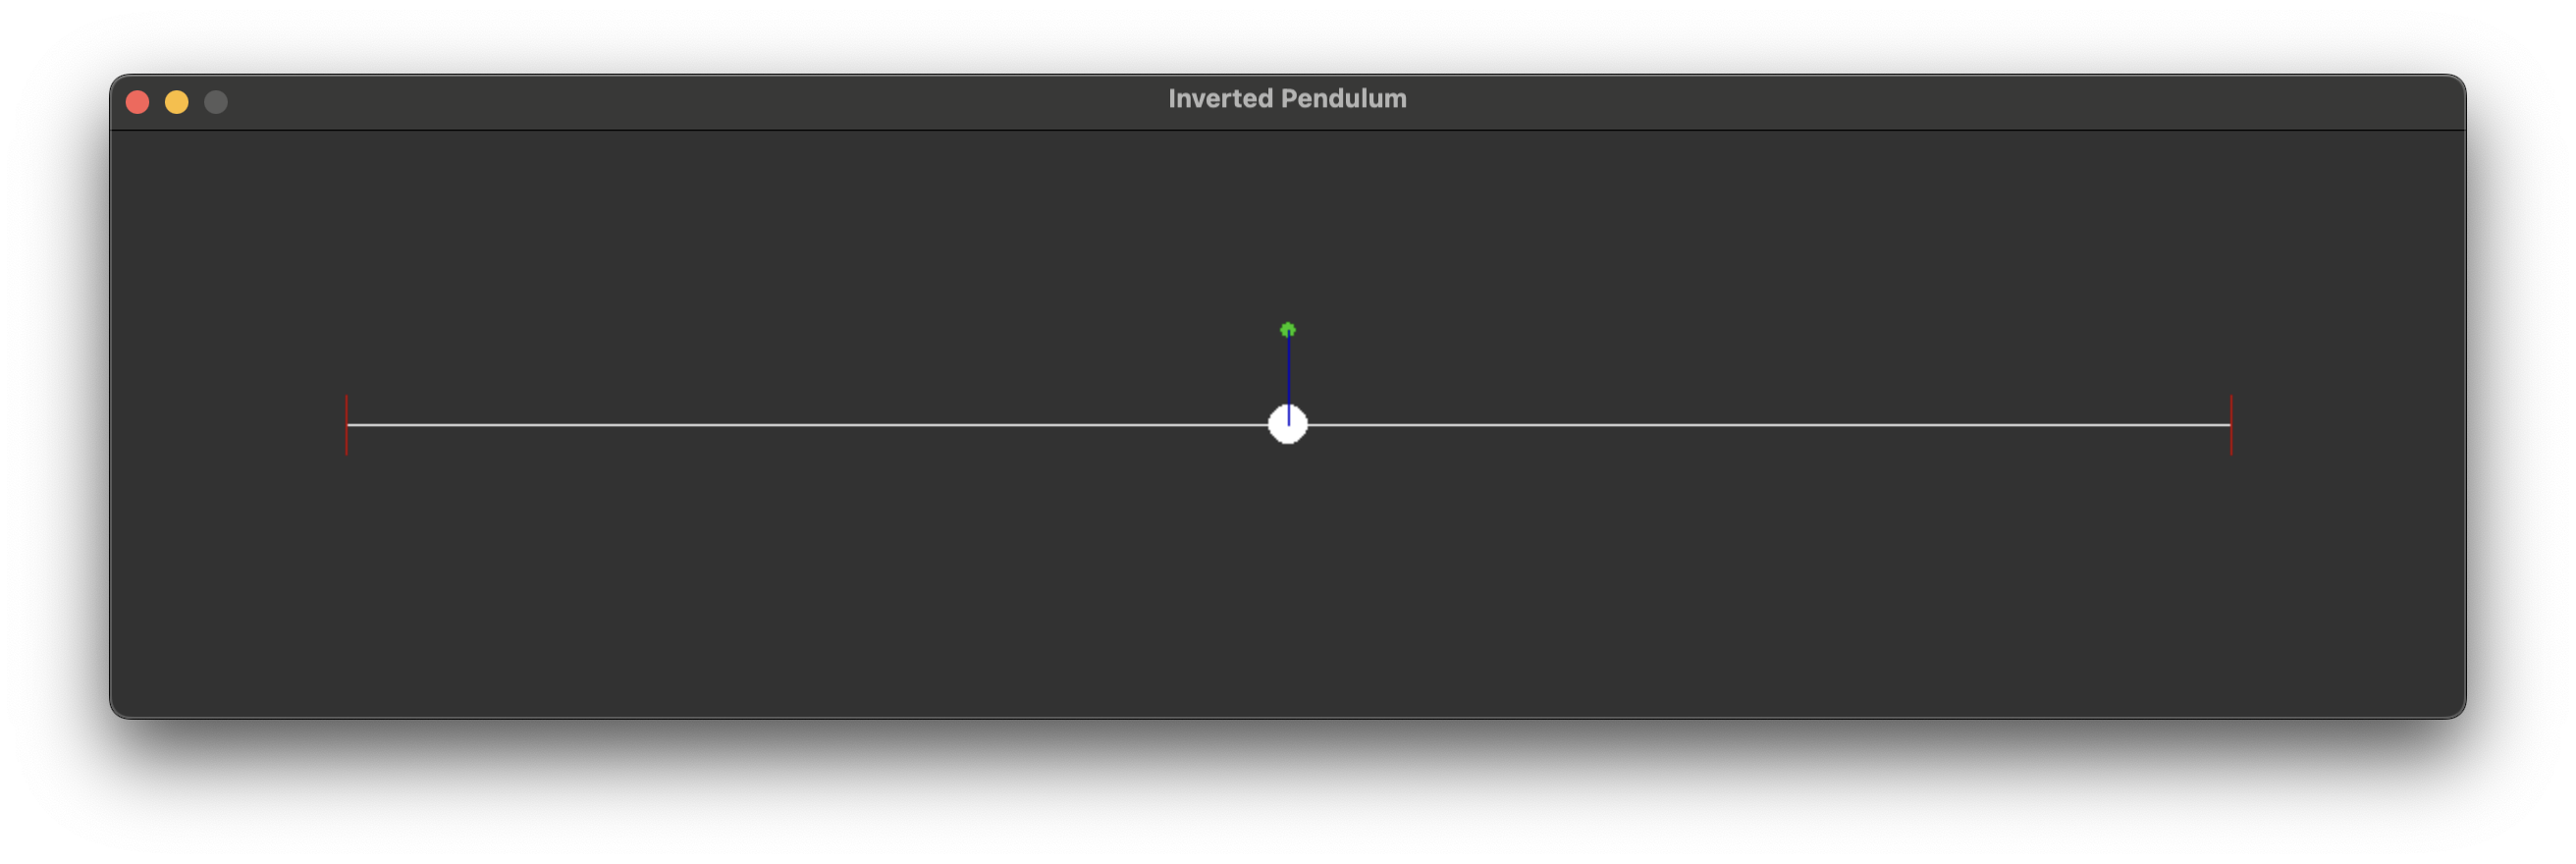
\includegraphics[width=\textwidth]{test_vis_1_1.png}
  \end{center}
  \caption{$x=0$ and $\theta=0$}
  \label{fig:test_vis_1_1}
\end{figure}

\begin{figure}[h!]
  \begin{center}
    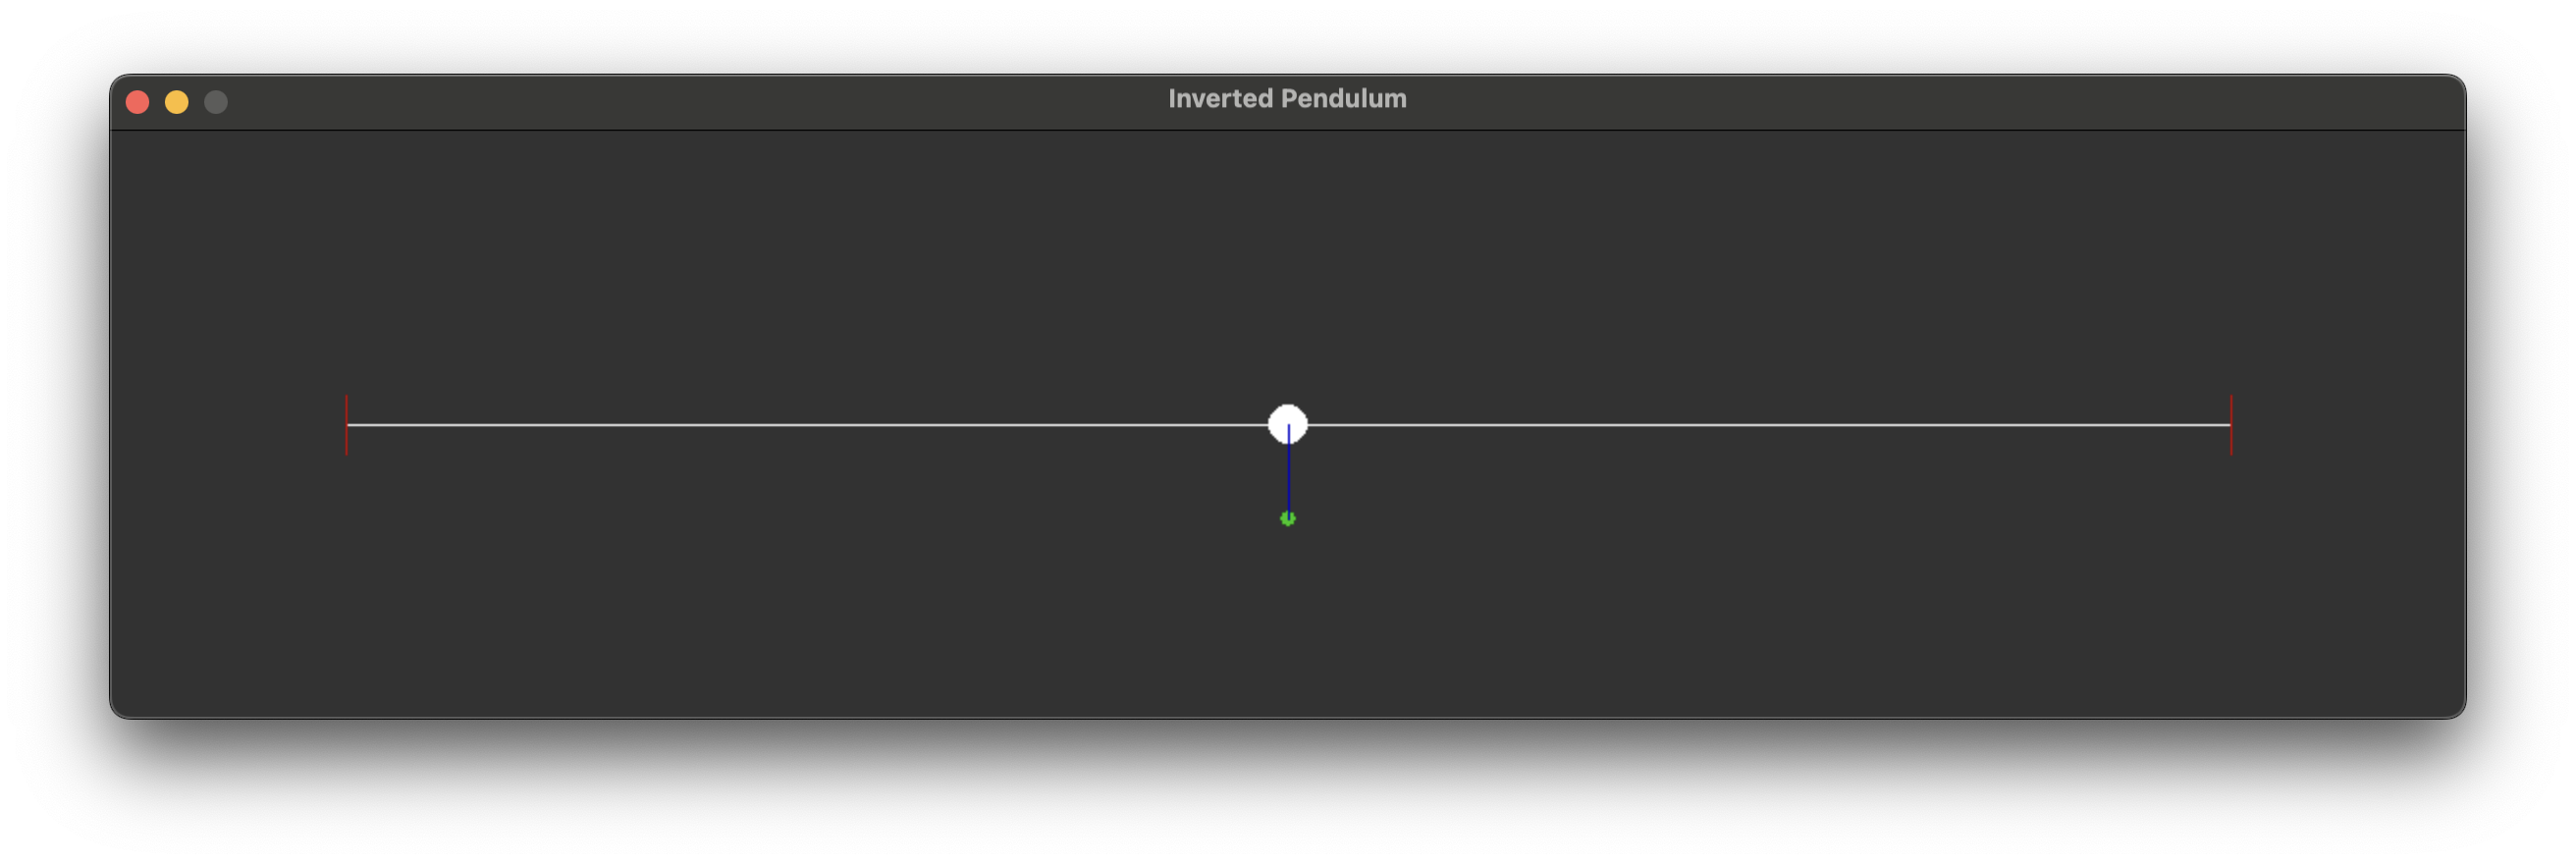
\includegraphics[width=\textwidth]{test_vis_1_2.png}
  \end{center}
  \caption{$x=0$ and $\theta=\pi$}
  \label{fig:test_vis_1_2}
\end{figure}

\begin{figure}[h!]
  \begin{center}
    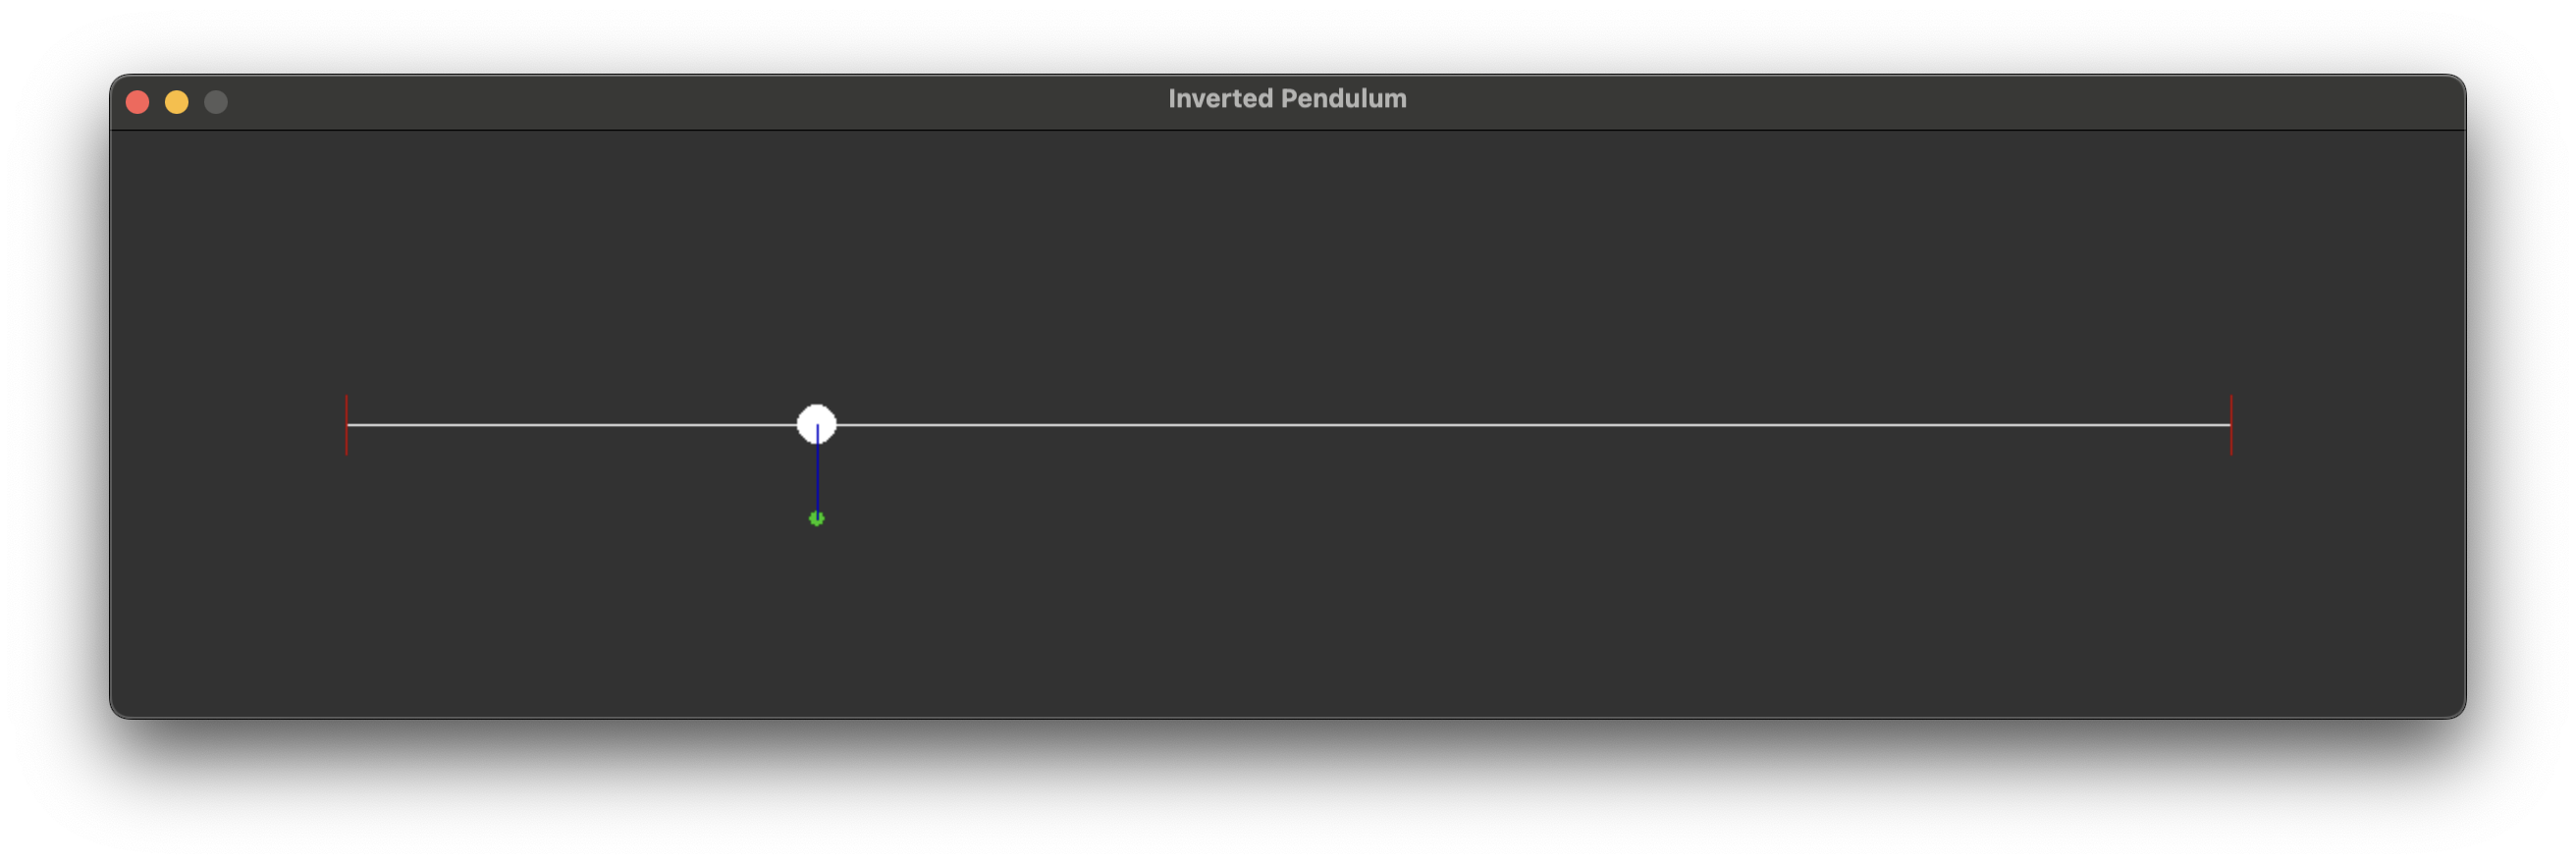
\includegraphics[width=\textwidth]{test_vis_1_3.png}
  \end{center}
  \caption{$x=-5$ and $\theta=\pi$}
  \label{fig:test_vis_1_3}
\end{figure}

\begin{figure}[h!]
  \begin{center}
    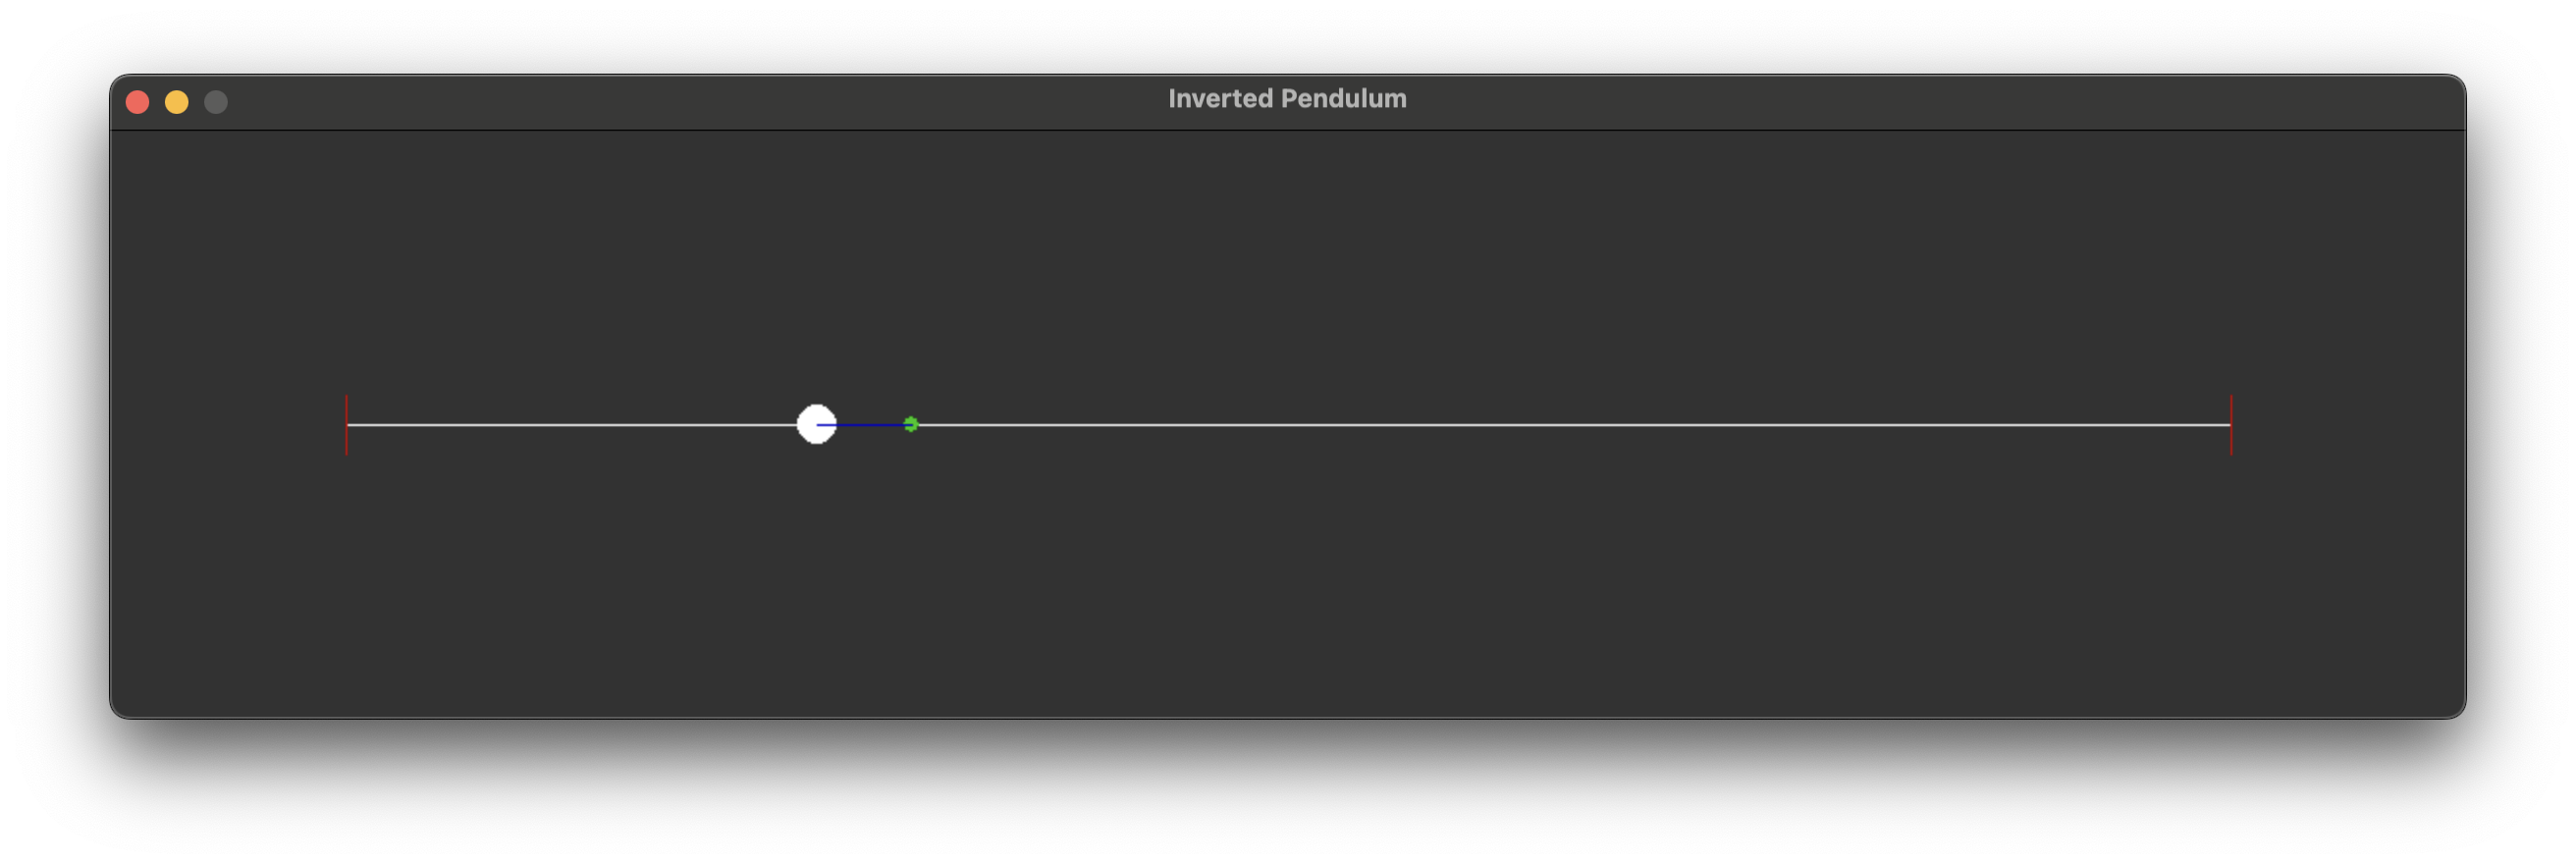
\includegraphics[width=\textwidth]{test_vis_1_4.png}
  \end{center}
  \caption{$x=-5$ and $\theta=\frac{\pi}{2}$}
  \label{fig:test_vis_1_4}
\end{figure}

\newpage

\section{Nonfunctional Requirements Evaluation}

\subsection{Usability}
		
\subsection{Performance}

\subsection{etc.}
	
\section{Comparison to Existing Implementation}	

This section will not be appropriate for every project.

\section{Unit Testing}

\section{Changes Due to Testing}

\wss{This section should highlight how feedback from the users and from 
the supervisor (when one exists) shaped the final product.  In particular 
the feedback from the Rev 0 demo to the supervisor (or to potential users) 
should be highlighted.}

\section{Automated Testing}
		
\section{Trace to Requirements}
		
\section{Trace to Modules}		

\section{Code Coverage Metrics}

\bibliographystyle{plainnat}
\bibliography{../../refs/References}

\newpage{}
\section*{Appendix --- Reflection}

The information in this section will be used to evaluate the team members on the
graduate attribute of Reflection.  Please answer the following question:

\begin{enumerate}
  \item In what ways was the Verification and Validation (VnV) Plan different
  from the activities that were actually conducted for VnV?  If there were
  differences, what changes required the modification in the plan?  Why did
  these changes occur?  Would you be able to anticipate these changes in future
  projects?  If there weren't any differences, how was your team able to clearly
  predict a feasible amount of effort and the right tasks needed to build the
  evidence that demonstrates the required quality?  (It is expected that most
  teams will have had to deviate from their original VnV Plan.)
\end{enumerate}

\end{document}